\documentclass[a4paper]{article}
\usepackage{listings}
\usepackage[T2A]{fontenc}
\usepackage[utf8]{inputenc}
\usepackage[ukrainian]{babel}
\usepackage{tikz}
\usepackage{lastpage} 
\usepackage[left=2.5cm, right=1.5cm, top=1.5cm, bottom=2.5cm]{geometry}
\usepackage{fancyhdr}
% \usepackage{graphicx}

\pagestyle{fancy}
\fancyhf{}
\renewcommand{\headrulewidth}{0pt}
\renewcommand{\footrulewidth}{0pt}
% \pagestyle{empty}

\newcommand{\makrosTitle}[2]{
\thispagestyle{empty}
        \centering
        \textbf{Міністерство освіти і науки України}\\
        \textbf{КИЇВСЬКИЙ ПОЛІТЕХНІЧНИЙ УНІВЕРССИТЕТ}\\[2cm]
        \raggedleft
        Кафедра автоматизації та систем неруйнівного контролю\\
        Група ПМ-11
        \vfill
        \centering
        \textbf{ПРОЕКТУВАННЯ СИСТЕМ АВТОМАТИЗАЦІЇ}\\[1cm]
        \textbf{ЗВІТ З ЛАБОРАТОРНОЇ РОБОТИ №#1}\\[1cm]
        \textbf{#2}
        \vfill
        \begin{flushleft}
            Керівник  \qquad\qquad\quad \hfill\qquad (підпис)\hfill 
            д.т.н., проф. Черепанська І. Ю.\\
            \hfill (дата)\\[2cm]
            Виконавець\hfill (підпис)\hfill Погорєлов Б. Ю.\\
            \hfill (дата)
        \end{flushleft}
        \vfill
        \centering
        2025
}

\newcommand{\makrosFrameBig}[2]{
    \thispagestyle{empty} % Вимикає номер сторінки на першій сторінці
    
    \begin{tikzpicture}[remember picture, overlay]
        \begin{scope}[shift={([xshift = 20 mm, yshift = 10 mm]current page.south west)}]
            \draw[line width=2] (0,0) rectangle (180 mm,277 mm);
        \end{scope}
    \end{tikzpicture}
    
    \begin{tikzpicture}[remember picture, overlay]
        \begin{scope}[shift={([xshift = 20 mm, yshift = 10 mm]current page.south west)}, x=1mm, y=1mm]
            \draw[line width=2] (0,0) rectangle (180,40);
            \draw[line width=2]  (7,40) -- (7, 25);
            \draw[line width=2] (17,40) -- (17, 0);
            \draw[line width=2] (40,40) -- (40, 0);
            \draw[line width=2] (55,40) -- (55, 0);
            \draw[line width=2] (65,40) -- (65, 0);
            \draw[line width=2] (135,25) -- (135,0);
            \draw[line width=2] (140,15) -- (140,20);
            \draw[line width=2] (145,15) -- (145,20);
            \draw[line width=2] (150,25) -- (150,15);
            \draw[line width=2] (165,25) -- (165,15);
        
            \draw (0,35) -- (65, 35);
            \draw[line width=2] (0,30) -- (65, 30);
            \draw[line width=2] (0,25) -- (180, 25);
            \draw (0,20) -- (65, 20);
            \draw (0,15) -- (65, 15);
            \draw (0,10) -- (65, 10);
            \draw (0,5) -- (65, 5);
        
            \draw[line width=2] (135,20) -- (180, 20);
            \draw[line width=2] (135,15) -- (180, 15);
            
            \node at (3.5, 27.5) {Зм.};
            \node at (12, 27.5) {Лист};
            \node at (28.5, 27.5) {№ докум.};
            \node at (47.5, 27.5) {Підпис};
            \node at (60, 27.5) {Дата};
            
            \node at (7, 22.5) {Розроб.};
            \node at (6.5, 17.5) {Перев.};
            \node at (8.5, 7.5) {Н. Контр.};
            \node[align=left] at (5, 2.5) {Затв.};
            
            \node at (142.5, 22.5) {Літ.};
            \node at (157.5, 22.5) {Аркуш};
            \node at (172, 22.5) {Аркушів};
        
            \node[align=left, font=\itshape, anchor=south west, scale=0.9] at (16, 20) {Погорєлов Б.Ю.};
            \node[align=left, font=\itshape, anchor=south west, scale=0.8] at (16, 15) {Черепанська І.Ю.};
            \node[align=left, font=\itshape, anchor=south west, scale=0.8] at (16, 0) {Черепанська І.Ю.};
        
            \node[anchor=center, font=\itshape, scale=1.5] at (122, 32) {#1};
            \node[align=center, font=\itshape, anchor=center] at (100, 12) {#2};
            \node[align=left, font=\itshape, anchor=south west, scale=0.9] at (135, 5) {КПІ ім. І. Сікорського, ПБФ};
            \node[anchor=center, font=\itshape] at (158, 17) {2};
            \node[anchor=center, font=\itshape] at (172, 17) {\pageref{LastPage}};    
        \end{scope} 
    \end{tikzpicture}
}

\newcommand{\makrosFrameSmall}[1]{
    % \thispagestyle{empty} % Вимикає номер сторінки на першій сторінці
    
    \begin{tikzpicture}[remember picture, overlay]
        \begin{scope}[shift={([xshift = 20 mm, yshift = 10 mm]current page.south west)}]
            \draw[line width=2] (0,0) rectangle (180 mm,277 mm);
        \end{scope}
    \end{tikzpicture}
    
    \begin{tikzpicture}[remember picture, overlay]
        \begin{scope}[shift={([xshift = 20 mm, yshift = 10 mm]current page.south west)}, x=1mm, y=1mm]
            \draw[line width=2] (0,0) rectangle (180,15);
            \draw[line width=2] (7,0) -- (7, 15);
            \draw[line width=2] (17,0) rectangle (43,15);
            \draw[line width=2] (55,0) rectangle (64,15);
            \draw[line width=2] (170,0) -- (170, 15);

            \draw[line width=2] (0,5) -- (64, 5);
            \draw               (0,10) -- (64, 10);
            \draw[line width=2] (170,8) -- (180, 8);

            \node[anchor=center, scale=0.8] at (3.5, 2.5) {Змн.};
            \node[anchor=center, scale=0.9] at (12, 2.5) {Арк.};
            \node[anchor=center] at (30, 2.5) {№~докум.};
            \node[anchor=center, scale=0.9] at (49, 2.5) {Підпис};
            \node[anchor=center, scale=0.9] at (59, 2.5) {Дата};
            \node[anchor=center, font=\itshape, scale=1.5] at (115, 7.5) 
                {#1};
            \node[anchor=center] at (175, 12) {Арк.};
            \node[anchor=center] at (175, 4) {\thepage};
            
        \end{scope}
    \end{tikzpicture}
}

% \makrosLab{1}{Шифр}{Назва}
\newcommand{\makrosLab}[3]{ 
    \fancyfoot[C]{\makrosFrameSmall{#2}}
    \makrosTitle{#1}{#3}
    \newpage
    \makrosFrameBig{#2}{#3}
    \raggedright
}


\begin{document}
    \makrosLab{1}{п}{
Розробка системи автоматизованого\\
або автоматичного керування \\
типовим технологічним об’єктом \\
за варіантами індивідуальних завдань.
    }
\section*{Тема роботи}
Розробка системи автоматизованого
або автоматичного керування 
типовим технологічним об’єктом 
за варіантами індивідуальних завдань.

\section*{Мета роботи}
Навчитися розробляти та складати структурні схеми
систем автоматичного або автоматизованого керування різними
технологічними об'єктами.

\section*{Порядок виконання роботи}
\begin{enumerate}
    \item Ознайомитись з теоретичними відомостями (пункт 1.2.)
    \item Вивчити та описати в загальному вигляді природутехнологічного об’єкту керування (ОК) і процеси, що протікають в ньому.
    \item Визначити та описати регульовані параметри, збурення і можливі дії керування.
    \item Скласти параметричну схему ОК із вказанням фізичних величин вхідних та вихідних сигналів і збурюючих впливів.
    \item Скласти структурну схему системи керування та описати її роботу в загальному вигляді.
    \item Зробити висновки по роботі та дати відповіді на контрольні питання (пункт 1.3).
    \item Оформити звіт згідно вимог (пункт 1.4).
\end{enumerate}

\newpage

\section*{Теоретичні відомості}

У рамках мого проєкту природно-технологічний об’єкт керування (ОК) можна описати як систему, яка включає інтегровані технології для ефективного збору, обробки та передачі сигналів у реальному часі в умовах автономної діяльності. ОК є комп'ютерним комплексом, здатним виконувати різноманітні завдання, від прийому і аналізу сигналів до управління безпілотними апаратами та іншими технологіями.

Процеси, що протікають в ОК, можна поділити на кілька етапів:

\begin{itemize}
    \item \textbf{Збір даних:} Комплекс здатний отримувати сигнали з різних джерел, таких як радіосигнали, GPS, камери та інші сенсори. Це дозволяє оперативно збирати інформацію про навколишнє середовище або інші пристрої, з якими взаємодіє система.
    \item \textbf{Обробка даних:} Програмне забезпечення на основі відкритих технологій обробляє отриману інформацію, виконуючи різні операції, такі як фільтрація, аналіз, дешифрування, порівняння з базою даних або алгоритмами машинного навчання. Оброблені дані можуть використовуватися для прийняття рішень або передачі інформації далі.
    \item \textbf{Передача даних:} ОК має модулі для передачі даних на інші пристрої або сервери, зокрема через мережі Wi-Fi, Bluetooth, LoRa та інші способи зв'язку, що забезпечує надійний зв'язок та координацію дій у польових умовах.
    \item \textbf{Управління пристроями:} ОК також дозволяє здійснювати управління різноманітними пристроями, такими як безпілотні апарати або інші автономні системи. В залежності від завдань, можуть застосовуватись різні алгоритми для забезпечення точності та ефективності дій.
    \item \textbf{Забезпечення безпеки:} Враховуючи використання відкритих технологій, система також реалізує високий рівень безпеки даних, що включає захист від кібератак, шифрування та верифікацію інформації.
\end{itemize}

Таким чином, ОК в рамках проєкту є комплексною системою, яка інтегрує технології збору, обробки та передачі інформації для виконання різних завдань у реальному часі, забезпечуючи автономність і ефективність роботи в польових умовах.

\begin{figure}[h]
    \centering
    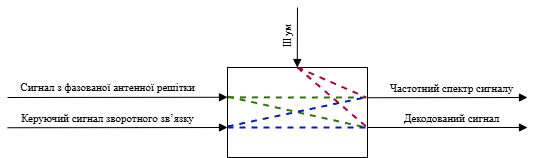
\includegraphics[width=0.7\textwidth]{imgs/PW1.1.png}
    \caption*{Рис. 1.1: Параметрична схема ОК із вказаними вхідними та вихідними сигналами}
\end{figure} 

\textbf{Вхідні параметри:}


\begin{itemize}
    \item \textbf{Сигнал з фазованої антенної решітки:} ОК використовує фазовану антенну решітку для прийому радіосигналів. Ця технологія дозволяє точно націлювати антену на джерело сигналу та знижувати рівень впливу небажаних перешкод, що важливо для забезпечення точності та надійності системи.
    \item \textbf{Керуючий сигнал зворотного зв'язку:} Зворотній зв'язок є важливим елементом в системі управління ОК. Керуючий сигнал дозволяє коригувати параметри роботи системи в реальному часі, забезпечуючи адаптацію до змінних умов навколишнього середовища та максимальну ефективність роботи.
\end{itemize}

\textbf{Збурення:}

\begin{itemize}
    \item \textbf{Радіо шуми:} Вхідні сигнали можуть бути піддані різним завадам, таким як радіо шуми, які можуть виникати через атмосферні явища або інші джерела перешкод. ОК має алгоритми для фільтрації та зменшення впливу шумів на якість сигналу.
    \item \textbf{Пристрої радіоелектронної боротьби:} ОК може бути підданий впливу пристроїв радіоелектронної боротьби, які намагаються заглушити або спотворити прийняті сигнали. Для подолання таких загроз система використовує методи активного та пасивного захисту, а також спеціалізовані алгоритми для виявлення та нейтралізації цих впливів.
\end{itemize}

\textbf{Вихідні параметри:}

\begin{itemize}
    \item \textbf{Частотний спектр сигналу:} ОК проводить аналіз сигналу для визначення його частотного спектру, що дозволяє виявляти характеристики сигналу, його джерело та можливі модифікації, спричинені завадами.
    \item \textbf{Декодований сигнал:} Після обробки отриманого сигналу ОК виконує декодування, що дозволяє відновити оригінальну інформацію. Для цього використовуються алгоритми дешифрування, які гарантують точність та швидкість відновлення даних.
\end{itemize}

\begin{figure}[h]
    \centering
    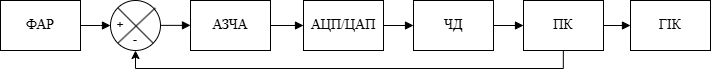
\includegraphics[width=1\textwidth]{imgs/PW1.2.png}
    \caption*{Рис. 1.2: Структурна схема}
\end{figure} 

\section*{Структурна схема керування}

Структурна схема керування описує взаємодію основних компонентів системи, починаючи з фазованої антенної решітки і закінчуючи графічним інтерфейсом користувача. Нижче наводиться опис кожного з елементів цієї схеми.

\begin{itemize}
    \item \textbf{ФАР (фазована антена решітка):} 
    Першим етапом у системі є фазована антенна решітка, яка використовується для прийому радіосигналів з високою точністю. Ця технологія дозволяє керувати напрямком прийому сигналу без необхідності фізичного повертання антени, що підвищує швидкість та ефективність обробки сигналу. Фазована антенна решітка забезпечує високі параметри чутливості та можливість зменшення впливу перешкод.
    
    \item \textbf{АЗЧА (апаратне забезпечення частотної адаптації):} 
    Далі сигнал проходить через апаратне забезпечення частотної адаптації, яке здійснює налаштування системи на конкретну частоту прийому. Це важливий етап для забезпечення стабільної роботи в умовах змінного радіочастотного середовища. Адаптація дозволяє коригувати частотні характеристики системи для ефективної обробки сигналу.
    
    \item \textbf{АЦП/ЦАП (аналого-цифровий і цифрово-аналоговий перетворювачі):} 
    Для перетворення сигналу в цифрову форму використовується аналого-цифровий перетворювач (АЦП). Сигнал після проходження адаптації подається на АЦП, який перетворює аналоговий сигнал у цифровий для подальшої обробки. Після обробки сигнал може бути повернутий у аналогову форму за допомогою цифро-аналогового перетворювача (ЦАП), якщо це необхідно для подальшого використання.
    
    \item \textbf{ЧД (частотна дискретизація):} 
    Після перетворення сигналу в цифрову форму здійснюється частотна дискретизація. Це процес, при якому сигнал розбивається на окремі дискретні значення, що дозволяє ефективно обробляти його за допомогою цифрових методів. Дискретизація дає змогу аналізувати сигнал у часовій області з необхідною точністю для подальших обчислень.
    
    \item \textbf{ПК (персональний комп'ютер):} 
    Обробка даних здійснюється на комп'ютері, що виконує алгоритми для фільтрації, аналізу та декодування отриманого сигналу. Комп'ютерна система виконує обчислення на основі отриманих цифрових даних, використовуючи спеціалізоване програмне забезпечення для обробки сигналів. Це дозволяє швидко отримувати точну інформацію та здійснювати необхідну адаптацію.
    
    \item \textbf{ГІК (графічний інтерфейс користувача):} 
    Результати обробки сигналу відображаються на графічному інтерфейсі користувача, що дає можливість оператору здійснювати моніторинг і контроль процесів в реальному часі. Інтерфейс надає зручний доступ до результатів обробки даних, надаючи оператору необхідну інформацію для прийняття рішень та коригування налаштувань системи.
\end{itemize}


\section*{Висновки}
Розроблена система дозволяє автоматично розпізнавати сигнали та передавати керуючі команди. Отримані результати підтверджують ефективність використання HACERFOne та Raspberry Pi для автоматизованого керування.

\section*{Відповіді на контрольні питання}
\begin{enumerate}
    \item \textbf{Що таке система автоматичного керування?}\\
    Це система, що здійснює керування технологічним об'єктом без участі оператора.
    \item \textbf{В чому полягає процес функціонування САК?}\\
    Система аналізує вхідні сигнали, обробляє їх та формує вихідний керуючий сигнал для об'єкта.
    \item \textbf{Основні терміни:}\
    \textbf{Система} – сукупність взаємопов'язаних елементів, що виконують певну функцію.\\
    \textbf{Об’єкт} – елемент, що підлягає керуванню.\\
    \textbf{Регулятор} – пристрій, що формує керуючий вплив.\\
    \textbf{Виконавчий механізм} – пристрій, що здійснює фізичну реалізацію керуючого впливу.\\
    \textbf{Регулювальний орган} – елемент, що змінює параметри об'єкта.\\
    \textbf{ТОК} – технологічний об'єкт керування.
    \item \textbf{З яких елементів складається система автоматичного керування?}\\
    Система складається з датчиків, контролера, виконавчих механізмів та керованого об'єкта.
\end{enumerate}


\end{document}